\documentclass[11pt]{article}
\usepackage[utf8]{inputenc}
\usepackage{geometry}
\usepackage{graphicx}
\usepackage{hyperref}
\usepackage{amsmath}
\usepackage{listings}
\usepackage{xcolor}
\usepackage{float}

% Set page margins
\geometry{a4paper, margin=1in}

% Set up code listing style
\lstset{
    basicstyle=\ttfamily,
    commentstyle=\color{gray},
    keywordstyle=\color{blue},
    stringstyle=\color{red},
    showstringspaces=false,
    captionpos=b
}

\title{Development of a Sudoku Solver: C1 Research Computing Coursework}
\author{Vishal Jain}
\date{\today}

\begin{document}

\maketitle

\tableofcontents

\newpage

\section{Introduction}

\begin{quote}
    "Sudoku is a denial of service attack on human
  intellect" - Ben Laurie
\end{quote}

This report details the development of a Sudoku solver inline with the requirements of the C1 Research Computing coursework. The programme takes as input an incomplete grid in the form of a text file with a 9x9 grid of numbers with zero representing unknown values and `|`,`+`,`-` separating cells and , i.e.:


\begin{verbatim}
    $ cat input.txt
    000|007|000
    000|009|504
    000|050|169
    ---+---+---
    080|000|305
    075|000|290
    406|000|080
    ---+---+---
    762|080|000
    103|900|000
    000|600|000
    \end{verbatim}

and outputs the completed grid in the same form.

\section{Problem Decomposition}
To architect the Sudoku solver program, an initial flowchart was constructed to map out the high-level logical sequence. Each step of the flowchart was assigned a color based on its logical independence. This method helped identify distinct, modular components within the program's workflow. The resulting color-coded flowchart is presented in Figure \ref{fig:solver_flowchart}.
\begin{figure}[H]
\centering
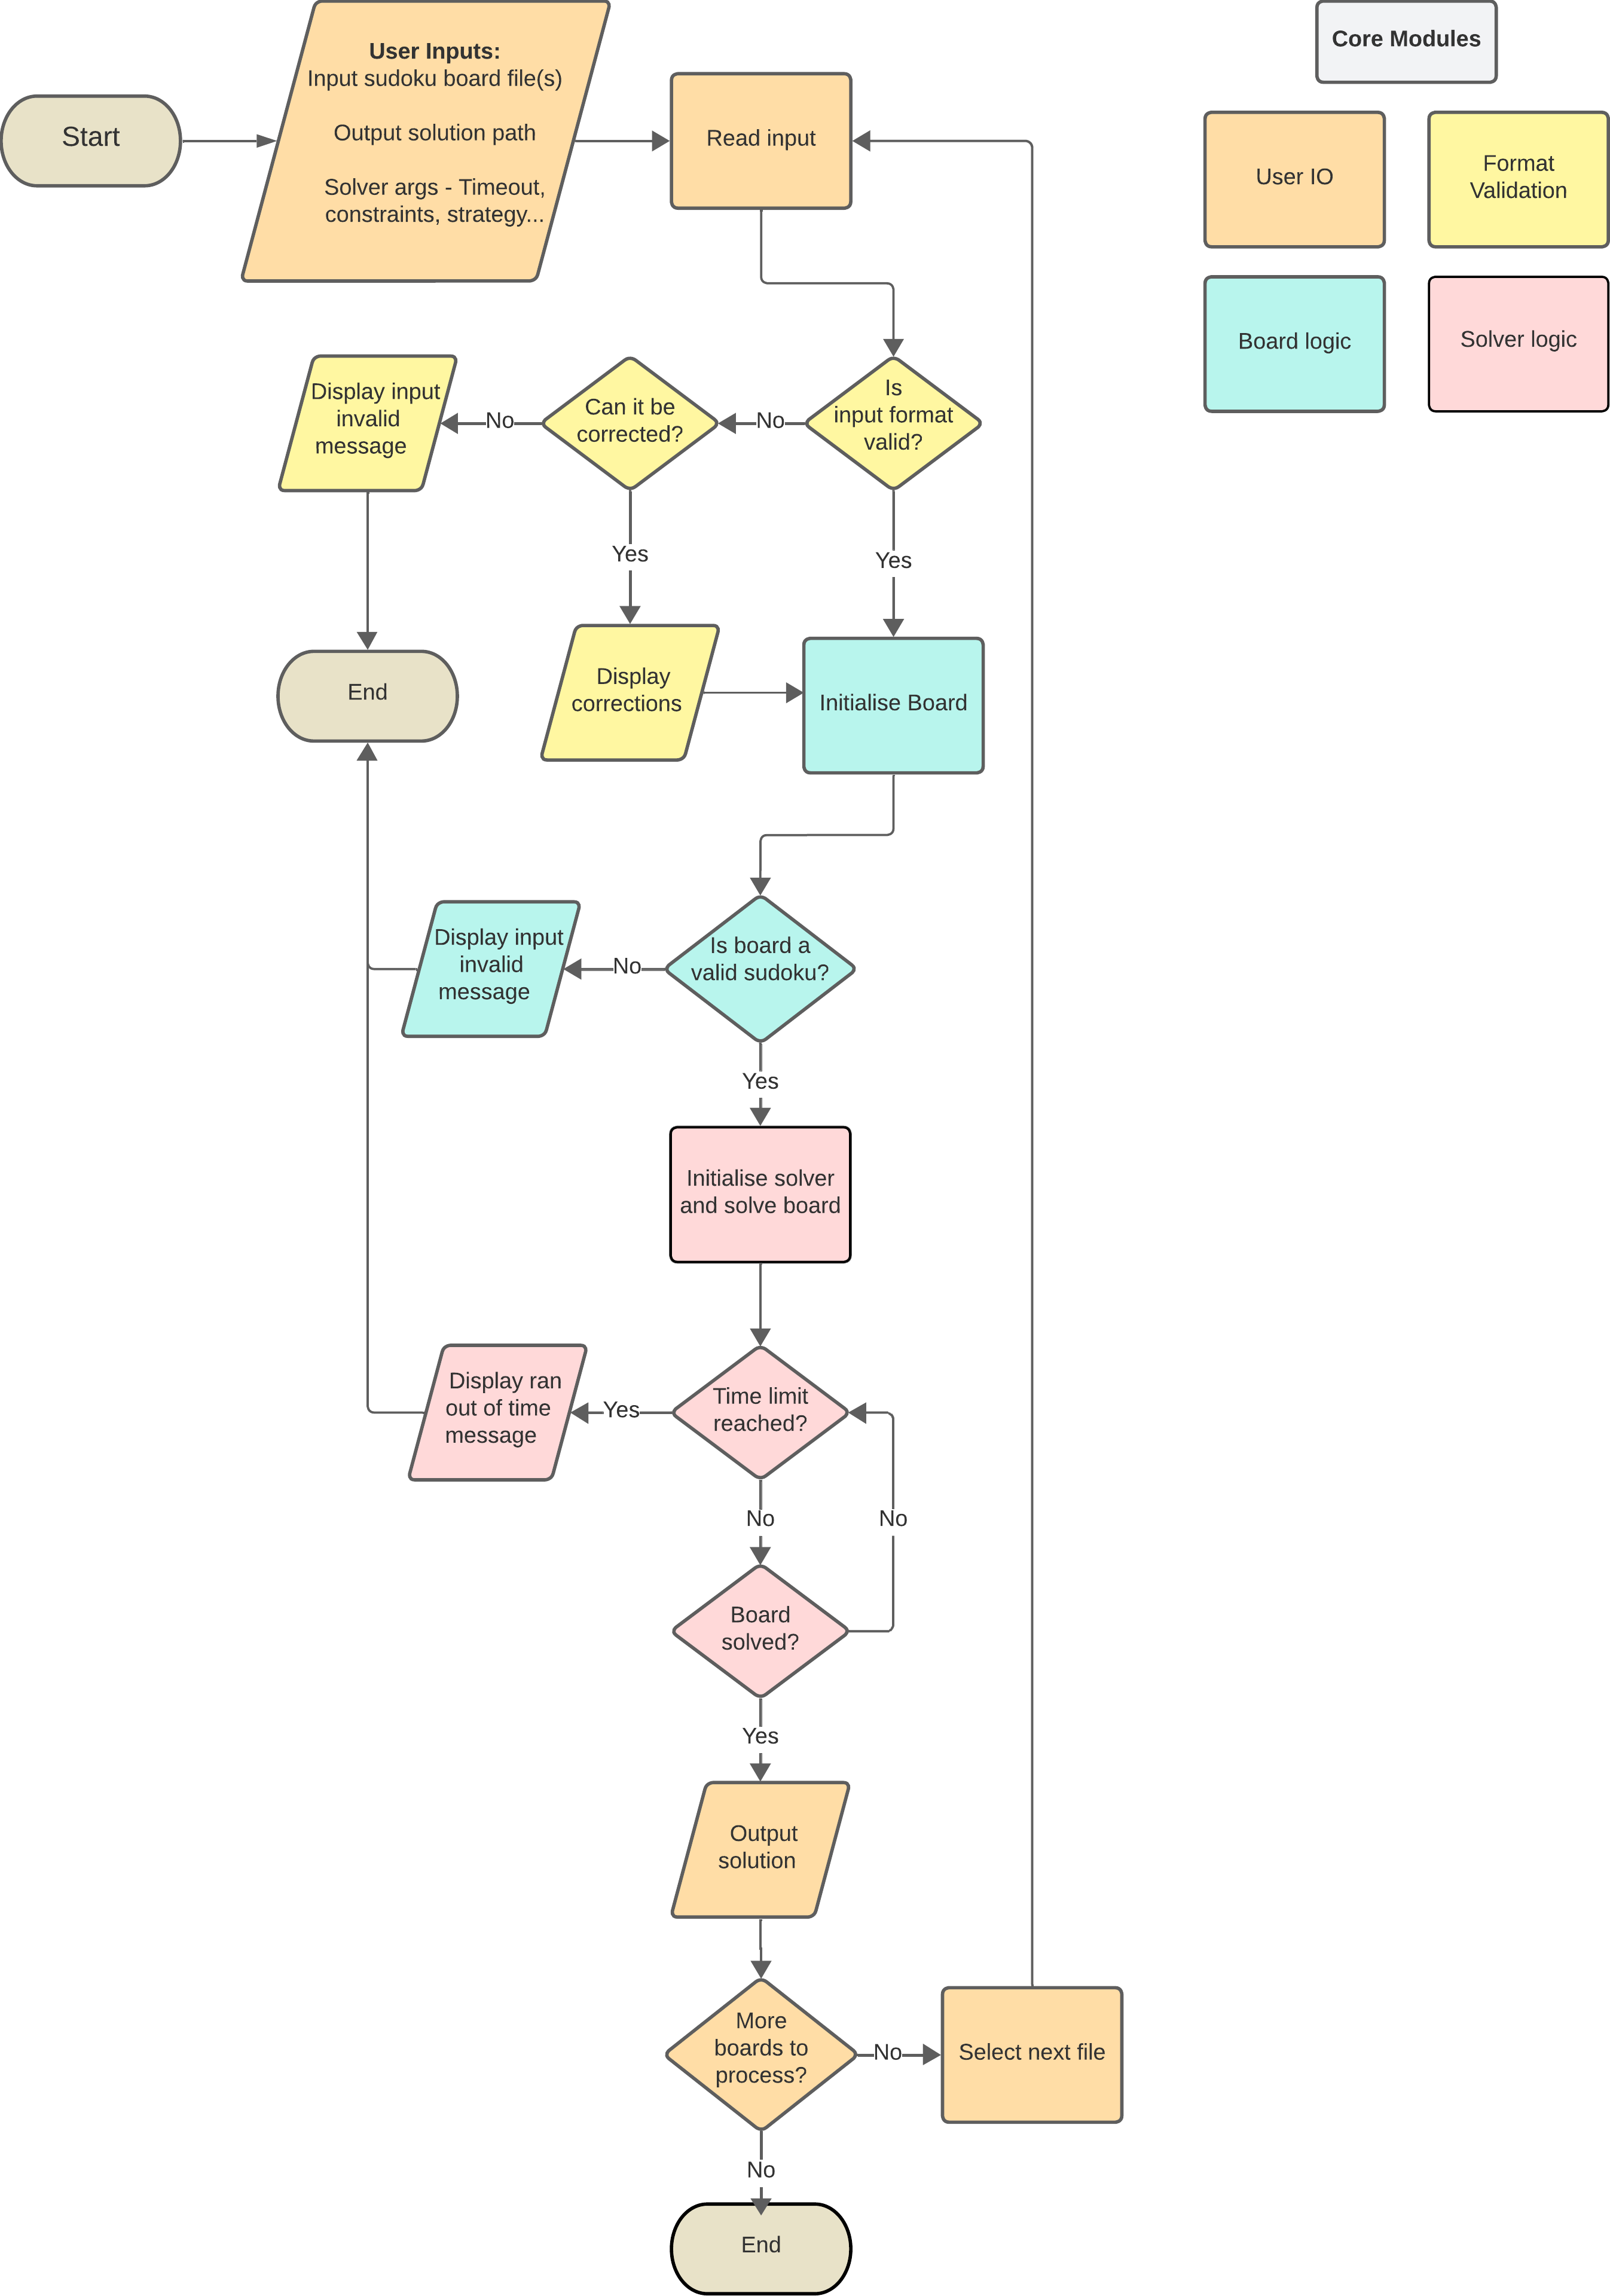
\includegraphics[width=1\textwidth]{figs/solver_flowchart.png}
\caption{High-level flowchart of the Sudoku solver program, illustrating the initial conceptual design. Functionally related modules are color-coded: orange for user interaction, yellow for format validation, cyan for board logic, and pink for solver logic components.}
\label{fig:solver_flowchart}
\end{figure}

The analysis led to the identification of the following key modular components in the Sudoku solver:

\begin{itemize}
\item \textbf{User IO:} Responsible for user interaction and input/output processing.
\item \textbf{Format Validation:} Ensures the correctness of the input format.
\item \textbf{Board Logic:} Manages the internal representation and manipulation of the Sudoku board.
\item \textbf{Solver Logic:} Implements the algorithms to solve the Sudoku puzzle.
\end{itemize}


\subsection{Developmental Journey}
Before delving into the final structure of the Sudoku solver, it is insightful to explore the initial prototyping phase. This phase laid the groundwork for the project and provided key insights that shaped the final design.

\subsubsection{Early Prototyping}
In the initial stages, the envisioned usage of the program was conceptualised as a straightforward sequence of operations involving board validation, board representation, and solving. The logical flow was as follows:

\begin{enumerate}
\item \textbf{Board Validation}: The user provides a file containing the Sudoku puzzle, which is then read, validated, and corrected if necessary. This process was handled by a utility function, \texttt{validate\_board}, located in the \texttt{utils} module. The function's purpose was to ensure the input adhered to Sudoku format standards and to correct any discrepancies. The code snippet for this step:
\begin{verbatim}
board_array = utils.validate_board(board_file)
\end{verbatim}
This function returns a 9x9 array representing the initial state of the Sudoku board.

\item \textbf{Board Representation}: The returned board array is then used to initialise an instance of the `\texttt{SudokuBoard}` class. This class encapsulates the board's representation and manipulation logic, providing common game board methods like `\texttt{reset}` and `\texttt{check\_valid}`. The initialisation step is shown below:
\begin{verbatim}
sudoku_board = SudokuBoard(board_array)
\end{verbatim}

\item \textbf{Solving the Puzzle}: Finally, the `\texttt{SudokuBoard}` instance is passed to the `\texttt{solve}` method of a `\texttt{BacktrackingSolver}` class instance. The solver applies the backtracking algorithm to find a solution to the puzzle, returning a new `\texttt{SudokuBoard}` instance representing the solved board:
\begin{verbatim}
solver = BacktrackingSolver().solve(board)
\end{verbatim}

\end{enumerate}


\subsubsection{Early Hurdles and Insights in Sudoku Solver Development}

\paragraph{Key Challenges and Evolutions}
\begin{itemize}
    \item \textbf{Modularity Challenges:} Initially, the program used a single function \texttt{validate\_board} for board validation, correction, and parsing, limiting flexibility and complicating the handling of different input formats.
    
    \item \textbf{Supporting Multiple Input Formats:} The solver encountered difficulties with non-grid formats, like Kaggle's single line format. This highlighted the need for native support for various formats and a more efficient approach to format conversion.

    \item \textbf{Evolution of SudokuBoard:} The \texttt{SudokuBoard} class was refined to focus solely on representing the board and interfacing with solvers, taking over some validation responsibilities and dropping output logic for a cleaner design.

    \item \textbf{Solver Extensibility:} The initial design did not easily accommodate different solver algorithms, especially those with unique initialisation needs. This led to an understanding of the necessity for a more flexible system for integrating new solvers.

    \item \textbf{Enhancing Input Flexibility in main.py:} Modifications were made to \texttt{main.py} to handle both single puzzle file paths and directories containing multiple puzzles. It also gained the capability for string input for quick puzzle testing and dynamic solver and format handler selection.
\end{itemize}


\subsubsection{High-Level Overview of the Final Implementation}
The final design of the Sudoku solver program encapsulates a modular and flexible architecture, as outlined below:

\begin{verbatim}
# Initialise the Format Handler and Solver
format_handler = SudokuFormatHandler()
solver = SudokuSolver()

# Parse the Sudoku board from the given input in the desired format
board = format_handler.parse(board_file, format_type)

# Employ a specific solver to find a solution for the parsed board 
solved_board = solver.solve(board, solver_backend)

# Save the solved board in the desired format and output path
format_handler.save(solved_board, format_type, output_path)
\end{verbatim}

In this design, \texttt{SudokuFormatHandler} and \texttt{SudokuSolver} act as wrapper classes that have methods which allow the user to specify which format and solver backend they want to use, respectively. These classes utilise standardised methods to process and solve the Sudoku puzzle, irrespective of the specific format or solving algorithm used. This approach significantly enhances the extensibility of the program, allowing for the easy integration of new formats and solving methods without requiring changes to the \texttt{main.py} script. Additionally, the flexibility to save the output in either the native format of the input or any other specified format is achieved by adjusting the \texttt{format\_type} argument, further increasing the program's versatility and user-friendliness. The next section will explore the design and implementation of the various modules in greater detail.

\section{Programme Modules}
\subsection{Class SudokuFormatHandler}

\subsubsection{Scope}
The scope of the FormatHandler classes implemented in \texttt{src/sudoku\_format\_handler.py} is defined by its role in bridging the gap between external representations of Sudoku boards and standardised internal representation. Specifically, the scope of this class encompasses:

\begin{itemize}
\item \textbf{Parsing}: Handling the conversion of the input, whether it comes as a string or as a file path, into a standardised \texttt{SudokuBoard} object.

\item \textbf{Saving}: Conversely, the class also manages the conversion of \texttt{SudokuBoard} objects back into user-readable formats. 

\item \textbf{Format Validation and Correction}: This class is also where the developer defines any methods for validation checks and corrections to ensure that the input is in the expected format before parsing.
\end{itemize}

\subsubsection{Design}
The design of the \texttt{SudokuFormatHandler} class is centered around principles of modularity and extensibility, driven by the use of an abstract base class and a handler dictionary. Key design aspects include:

\begin{itemize}
    \item \textbf{Modularity}: The class leverages an abstract base class, \texttt{FormatHandler}, which outlines essential methods -- \texttt{parse} and \texttt{save}. This structure ensures consistency across different format handlers while allowing for flexibility in their specific implementations.
    \item \textbf{Extensibility}: New formats can be easily integrated into the system by creating a subclass of \texttt{FormatHandler} and adding it to \texttt{SudokuFormatHandler}'s \texttt{handler\_dict} class attribute. This approach simplifies the process of extending the system to accommodate new Sudoku board formats.
    \item \textbf{Abstraction}: The abstract methods in \texttt{FormatHandler} enforce a contract that all subclasses must provide specific implementations for parsing and saving Sudoku boards, thus maintaining a standardised interface.
\end{itemize}
The UML class diagrams in Figure \ref{fig:format_handler_uml} provide a visual representation of the design and implementation of the \texttt{FormatHandler} abstract base class and the \texttt{SudokuFormatHandler} class, respectively.
\begin{figure}[H]
    \centering
    \includegraphics[width=1\textwidth]{figs/UML_sudoku_handler.png}
    \caption{Class diagram for the SudokuFormatHandler module, illustrating the design and implementation of the FormatHandler abstract base class and the SudokuFormatHandler class. Along with the composition of the SudokuFormatHandler class with the implemented Format classes (GridFormatHandler and FlatFormatHandler).}
    \label{fig:format_handler_uml}
\end{figure}

\subsubsection{Implementation}
The implementation of \texttt{SudokuFormatHandler} involves several key components that collectively enable dynamic handling of various board formats:

\begin{itemize}
    \item \textbf{Handler Dictionary}: The \texttt{handler\_dict} serves as a central repository linking format types (e.g., 'grid', 'flat') to their corresponding handler objects, facilitating the flexible handling of different formats.
    \item \textbf{Handler Retrieval}: The method \texttt{\_get\_handler} takes a format type as input and retrieves the appropriate handler from \texttt{handler\_dict}. It raises a \texttt{KeyError} with available format options in case of an unsupported format type.
    \item \textbf{Parse Method}: The \texttt{parse} method interfaces with the selected handler to transform the input into a \texttt{SudokuBoard} object. It delegates the specifics of parsing to the corresponding format handler.
    \item \textbf{Save Method}: Similarly, the \texttt{save} method utilizes the appropriate handler to convert a \texttt{SudokuBoard} object back into a file, ensuring consistency in the output process across different input formats.
\end{itemize}

\paragraph{GridFormatHandler}
The GridFormatHandler is the format handler for the required format of this coursework. It is designed to handle the parsing and saving of Sudoku boards in the grid format. The parsing process involves reading the input file or string and converting it into a list of strings representing each row of the Sudoku board. The white space and empty lines are removed. Any dots are replacecd with zeros as this is commonly seen online as a placeholder for empty cells.The handler ensures there are exactly 11 rows; otherwise, it raises an error. Each row undergoes validation against a specific regex pattern. If a row deviates from the expected pattern but aligns with an alternate acceptable one, it undergoes correction; otherwise, an error is raised. Correction logic is applied selectively: Separator rows lacking numbers are replaced with a standard separator row, but if they contain numbers, an error is raised to avoid digit alteration. For a row which is expected to describe a number row, if it matches the general pattern of 3 sets of numeric character triplets seperated by a non numeric character, it is corrected by inserting the expected seperator characters between the triplets.

\subsubsection{Extensibility}
The\texttt{SudokuFormatHandler} is designed with extensibility in mind. To support a new format, a developer simply needs to create a new handler class extending \texttt{FormatHandler} and implement the \texttt{parse} and \texttt{save} methods with the expected inputs and outputs. The new handler can then be added to the \texttt{handler\_dict}. This design makes it straightforward to extend the solver's capabilities to accommodate future requirements or user preferences for different Sudoku board formats.


\subsubsection{Limitations}
The current design of the SudokuFormatHandler module, as well as other related modules, is specifically tailored to process single Sudoku boards from individual input files. This intentional design choice is due to the significant increase in complexity that would arise from trying to build a general framework which supports multiple formats that also supports accommodating multiple boards within a single file. Maintaining a single input, single board paradigm simplifies the overall program structure and aligns with our current functional objectives. 


\subsection{SudokuBoard Class}
Future work is to make a board abc for future representations like dictionary based boards

\subsubsection{Scope}
The \texttt{SudokuBoard} class in \texttt{src/sudoku\_board.py} is integral to managing the internal representation and manipulation of the Sudoku board and providing a standardised interface for the other classes in the program. The scope of this class encompasses:

\begin{itemize}
    \item \textbf{Board Validation}: Makes sure board state always follows Sudoku rules. 
    \item \textbf{Board Representation}: Provides a standardised representation of the board state for the other classes. 
    \item \textbf{Board Manipulation}: Facilitates methods for resetting the board and modifying cell values to allow for board manipulation.
    \item \textbf{Solving Assistance}: Provides common utility methods required by typical solvers, such as fetching empty cells and checking valid number placements.

\end{itemize}
\subsubsection{Design and implementation}
The design of the \texttt{SudokuBoard} class is centered around the principle of encapsulation. The other classes in the program interact with the board through a standardised interface defined by this classes methods. 
\begin{itemize}
    \item \textbf{Array like interface}: Practices encapsulation by hiding the underlying board array attribute and instead provides an interface to access elements through use of custom
    \texttt{\_\_getitem\_\_} and \texttt{\_\_setitem\_\_} methods, the \texttt{SudokuBoard}.
    \item \textbf{Board Representation and Validation}: It utilises a 2D numpy array for board representation and sets for efficient look up of numbers in rows, columns, and 3x3 subgrids. 

    \item \textbf{Convenience Methods}: The class offers methods for board state manipulation (reset, place number, remove number) and utility functions (get related cell values, find empty cells), simplifying common operations in Sudoku puzzle solving.
    
    \item \textbf{Initialisation and Formatting}: The \texttt{\_\_init\_\_} method initialises the board with a given state, handling type and value checks. The \texttt{\_\_str\_\_} method provides a formatted string representation of the board, improving readability.

\end{itemize}

The UMl class diagram in Figure \ref{fig:sudoku_board_uml} provides a visual representation of the implementation of the \texttt{SudokuBoard} class.

\begin{figure}[H]
    \centering
    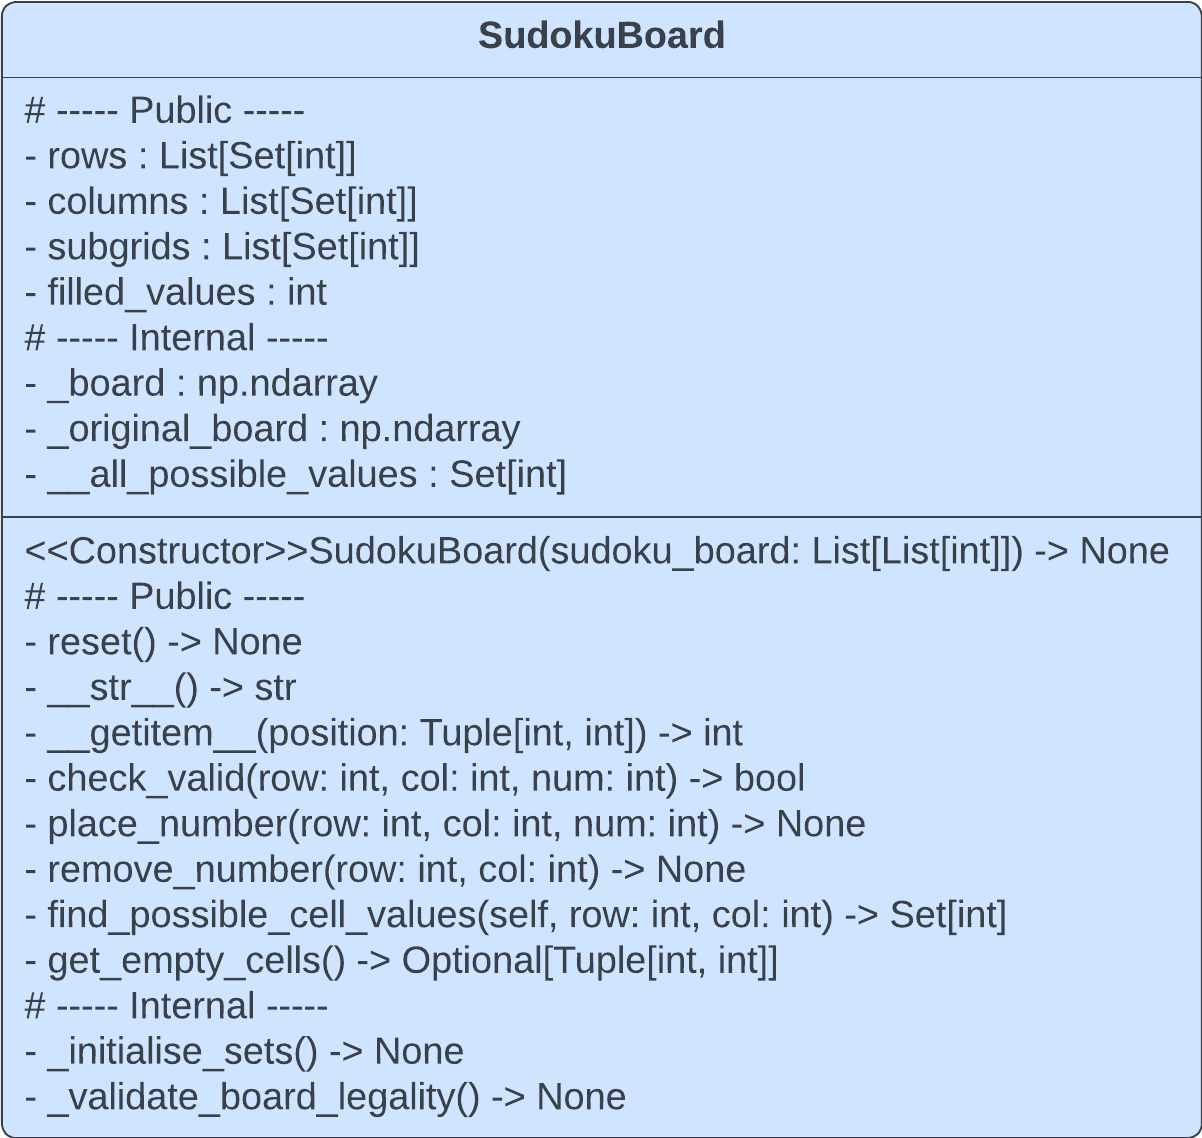
\includegraphics[width=0.6\textwidth]{figs/UML_sudoku_board.png}
    \caption{UML class diagram for the SudokuBoard module.}
    \label{fig:sudoku_board_uml}
\end{figure}
 
\subsubsection{Extensibility and Limitations}
The \texttt{SudokuBoard} class, unlike \texttt{SudokuFormatHandler}, isn't inherently extensible for different board types such as dictionary representations. To address this, an abstract \texttt{Board} base class could be introduced, defining methods for solvers and format handlers with standardised inputs and outputs. \texttt{SudokuBoard} would then extend this base, allowing for various concrete \texttt{Board} implementations to handle different representations.
\subsection{SudokuSolver Class}

\subsection{main.py}

\section {Testing and Optimisation}
\subsection {Profiling}

\section {SWE}
Unit Tests and CI set up
Packaging and Usability

\section {Summary}

% \subsection{Scope}
% The User IO module serves as the primary interface between the user and the Sudoku solver program. Its responsibilities include:

% \begin{itemize}
% \item Collecting user input.
% \item Validating user input.
% \item Displaying the output of the program.
% \item Saving the output of the program.
% \end{itemize}

% \subsection{Design Considerations}
% Contrary to the development order, the User IO module's design was influenced significantly by prior interaction with other modules. This sequential approach ensured a more user-centric design, accommodating the needs identified through initial module interactions.

% \subsubsection{User Input Flexibility}
% A key feature of this module is its flexibility in accepting user input, either directly as a string or via a filepath. This was driven by the practical need to quickly test Sudoku boards obtained from various sources, often online. Additionally, the design allows for effortless expansion to accommodate new solvers or input formats.

% \subsection{Operational Modes}
% The User IO module supports two primary modes of operation:

% \begin{itemize}
% \item \textbf{Single Input Mode}: For individual puzzle solving, this mode is optimised for ease of use, requiring minimal parameters.
% \item \textbf{Batch Testing Mode}: Geared towards performance analysis, this mode facilitates processing multiple puzzles from a directory, with options for output saving and detailed statistical analysis.
% \end{itemize}

% \subsection{Future Extensibility and Reproducibility}
% The current implementation of solvers is straightforward, with a single timeout parameter. However, the design anticipates more complex solvers in the future. A specific section in main.py is earmarked for integrating such enhancements, potentially through a configuration file mechanism.

% To aid in the reproducibility of runs, particularly for performance comparison across different solver versions, the module captures and stores the git commit hash and run arguments in the output summaries.

% \subsection{Implementation Strategy}
% The module is implemented as a set of functions in the main.py script, favoring function-based design over a class-based approach. This decision was driven by the need for rapid prototyping and ease of adding new features.

% A high level overview of the implementation is shown in figure
% \subsubsection{Argument Parsing}
% Using argparse, the script effectively handles various user inputs. The design ensures that the most straightforward use case—solving a single puzzle—requires the least user input. Additional options like output path and run statistics are available for deeper analysis. The batch mode is specifically tailored for performance testing, generating comprehensive statistical data for each puzzle in the dataset.


% \subsubsection{Backend Integration}
% As the backend evolves with new solvers and input formats, these enhancements are automatically integrated into the User IO module, demonstrating the system's extensible and user-centric architecture.
% Uncomment the following two lines if you have references
%\bibliographystyle{plain}
%\bibliography{references}

\end{document}
